% Please add the following required packages to your document preamble:
% \usepackage[table,xcdraw]{xcolor}
% If you use beamer only pass "xcolor=table" option, i.e. \documentclass[xcolor=table]{beamer}
\begin{table}[H]
\centering
\begin{tabular}{|l|l|c|}
\hline
\rowcolor[HTML]{CBCEFB} 
\multicolumn{1}{|c|}{\cellcolor[HTML]{CBCEFB}\textbf{Código}} & \multicolumn{1}{c|}{\cellcolor[HTML]{CBCEFB}\textbf{Caso de uso}} & \textbf{Horas Hombre} \\ \hline
CU01                                                          & Incluyendo un evento cultural                                     & 30                    \\ \hline
CU02                                                          & Eliminando un evento cultural                                     & 8                     \\ \hline
CU03                                                          & Buscando evento                                                   & 56                    \\ \hline
CU04                                                          & Rankeando evento                                                  & 60                    \\ \hline
CU05                                                          & Logueándose                                                       & 59                    \\ \hline
CU06                                                          & Compartiendo información en redes sociales                        & 8                     \\ \hline
CU07                                                          & Editando un evento cultural                                       & 8                     \\ \hline
CU08                                                          & Registrándose                                                     & 20                    \\ \hline
CU09                                                          & Verificando contenido inapropiado automáticamente                 & 48                    \\ \hline
CU10                                                          & Verificando contenido inapropiado manualmente                     & 8                     \\ \hline
CU11                                                          & Reservando hoteles                                                & 56                    \\ \hline
CU12                                                          & Reservando vuelos                                                 & 48                    \\ \hline
CU13                                                          & Enviando publicidad                                               & 20                    \\ \hline
CU14                                                          & Visualizando caminos                                              & 48                    \\ \hline
CU15                                                          & Realizando reserva                                                & 56                    \\ \hline
CU16                                                          & Filtrando resultados                                              & 20                    \\ \hline
CU17                                                          & Obteniendo estadísticas sobre los usuarios                        & 32                    \\ \hline
CU18                                                          & Combinando eventos                                                & 32                    \\ \hline
\end{tabular}
\caption{Casos de uso}
\label{tab:cu}
\end{table}

\subsection{Diagrama de Casos de uso}

\begin{figure}[H]
 \centering
  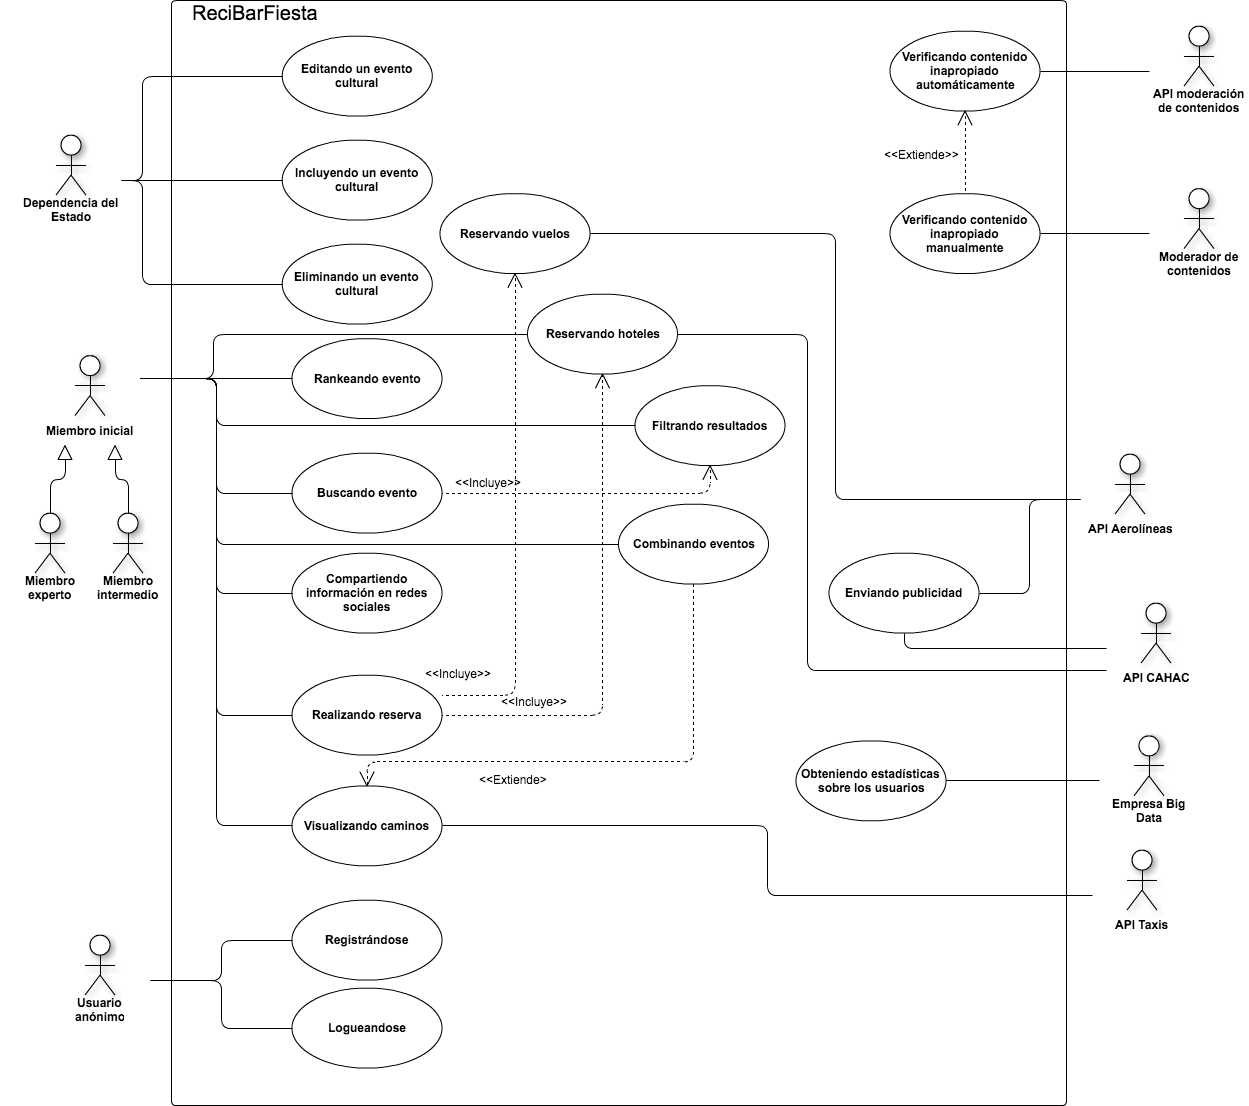
\includegraphics[width=\textwidth]{diagramas/casosDeUso.png}
  \caption{Diagrama de Casos de Uso de ReciBarFiesta}
  \label{fig:cu}
\end{figure}

\subsection{Descripción de los Casos de uso}
\begin{enumerate}
  \item \textbf{Incluyendo un evento cultural:} se refiere a la funcionalidad para agregar nuevos eventos, como recitales, charlas, festivales, etc. Solo lo pueden hacer usuarios autorizados (inicialmente solo miembros de dependencias del Estado).
  \item \textbf{Eliminando un evento cultural:} se refiere a la funcionalidad por la cual una dependencia del Estado puede eliminar un evento cultural previamente creado.
  \item \textbf{Editando un evento cultural:} se refiere a la funcionalidad por la cual una dependencia del Estado puede modificar los datos de un evento cultural previamente creado.
  \item \textbf{Rankeando evento:} se refiere a la funcionalidad que le permite a un miembro identificado de la comunidad calificar un evento en distintas categorías como, por ejemplo, ``Organización'', “Calidad” y “Ubicación”. Solo usuarios identificados podrán realizar esta acción, y se ponderará la calificación de acuerdo a la categoría del usuario (inicial, intermedio o experto).
  \item \textbf{Buscando evento:} se refiere a la funcionalidad por la cual los usuarios de la aplicación buscarán eventos, pudiendo filtrar los resultados por una serie de criterios (por ejemplo: fecha, temática, ubicación, etc) usando el caso de uso ``Filtrando resultados'' (CU16). Una descripción detallada puede hallarse en la tabla \ref{tab:cu05}.
  \begin{table}[H]
  \centering
  \begin{tabularx}{\textwidth}{|X|X|}
    \hline
    \rowcolor[HTML]{CBCEFB} 
    \multicolumn{2}{|l|}{\textbf{Caso de uso: Buscando evento}} \\ \hline
    \rowcolor[HTML]{CBCEFB}
    \multicolumn{2}{|l|}{Actor: Usuario de la Aplicación (básico, intermedio, avanzado, anónimo)} \\ \hline
    \rowcolor[HTML]{CBCEFB}
    \textbf{Curso Normal} & \textbf{Curso Alternativo} \\ \hline
    1) El usuario ingresa un texto en el buscador de eventos. & 1.1 El usuario en esta instancia puede agregar un filtro de modo que la búsqueda se realice ya con el filtro incluido. \\ \hline
    2) El sistema busca eventos cuyo nombre contenga o tenga una relación con el texto ingresado. & 2.1 Si el usuario escribió un texto con caracteres inválidos el sistema muestra un error y pide al usuario que ingrese nuevamente un texto. \\ \hline
    3) El sistema muestra los resultados obtenidos. Los resultados se muestran en una  lista con los eventos y los links que lleven a las vistas detalladas de cada uno de ellos. Además, & 3.1 Si el sistema no encuentra resultados para el texto ingresado, muestra la vista de resultados vacía con un mensaje informando que no hubo resultados para el texto ingresado. (Fin del caso) \\ \hline
    4) El usuario puede agregar un filtro a la la lista de resultados: fecha, temática, ubicación, etc.  seleccionando el filtro correspondiente y con su valor asociado (según el tipo de filtro) (CU14: Filtrando eventos) & \\ \hline
    5) El sistema filtra y muestra los resultados según el filtro configurado. &  \\ \hline
    6) Fin del caso & \\
    \hline
  \end{tabularx}
  \caption{Descripción detallada de CU05:Buscando evento}
  \label{tab:cu05}
  \end{table}
  \item \textbf{Compartiendo información en redes sociales:} se refiere a la funcionalidad por la cual los miembros de la comunidad podrán compartir los diferentes eventos disponibles en la aplicación en diferentes redes sociales como Facebook o Twitter, de manera que otras personas que no necesariamente tienen la aplicación puedan conocer su existencia.
  \item \textbf{Logueandose:} se refiere a la funcionalidad por la cual los usuarios anónimos con una cuenta previamente creada podrán identificarse con el sistema, lo cual les habilitará a tener información personalizada (por ejemplo, según el barrio en el que viven), valorar eventos, y poder realizar reservas de vuelos y hoteles.
  \item \textbf{Registrándose:} se refiere a la funcionalidad a través de la cual los usuarios anónimos pueden crearse una cuenta en el sistema, para eventualmente poder identificarse y aprovechar los privilegios que esto acarrea.
  \item \textbf{Verificando contenido inapropiado automatizado:} se refiere a la funcionalidad con la que el sistema utiliza la API de moderación de contenidos. La misma pone puntajes de 1 (contenido inapropiado), 2 (contenido dudoso, proceder a verificación manual) o 3 (contenido seguro)
  \item \textbf{Verificando contenido inapropiado manualmente:} se refiere a la funcionalidad para que un moderador pueda determinar si un determinado contenido es apropiado o no. Este caso de uso solo se activa para aquellos contenidos que son calificados con 2 por CU9.
  \item \textbf{Enviando Publicidad:} se refiere a la funcionalidad que le permite a los sponsors económicos de la aplicación enviar su material publicitario para ser mostrado por la página.
  \item \textbf{Visualizando Caminos:} se refiere a la funcionalidad que permite a los usuarios visualizar el o los caminos (en caso de que se hayan seleccionado múltiples eventos) desde su posición actual hasta cada evento. Se ofrecen diferentes tipos de rutas: caminando, en auto particular, en taxi (usando la aplicación del gobierno de la Ciudad), y en transporte público. Eventualmente pueden combinarse eventos (CU18).
  \item \textbf{Reservando Hoteles:} se refiere a la funcionalidad por la cual la API del sistema de la Cámara de Hoteles y Afines de la Ciudad (CAHAC) podrá registrar reservas de hoteles efectuadas por usuarios de la aplicación.
  \item \textbf{Reservando Vuelos:} se refiere a la funcionalidad por la cual la API del sistema de Aerolíneas Argentinas podrá registrar reservas de vuelos efectuadas por usuarios de la aplicación.
  \item  \textbf{Obteniendo estadísticas sobre los usuarios:} se refiere a la API desarrollada para que las empresas de Big Data puedan obtener los datos estadísticos sobre los usuarios.
  \item  \textbf{Filtrando resultados:} se refiere a la funcionalidad que le permite a los usuarios de la aplicación filtrar listas de eventos según diversos criterios a determinar.
  \item  \textbf{Realizando Reserva:} se refiere a la funcionalidad por la cual los miembros de la comunidad podrán seleccionar y reservar vuelos/hoteles para participar de eventos publicados en la aplicación utilizando los servicios provistos por Aerolíneas Argentinas, para vuelos, y de la Cámara de Hoteles y Afines de la Ciudad, para alojamientos. Una descripción detallada de este caso de uso puede encontrarse en la tabla \ref{tab:cu17}.
  \begin{table}[H]
  \centering
  \begin{tabularx}{\textwidth}{|X|X|}
    \hline
    \rowcolor[HTML]{CBCEFB} 
    \multicolumn{2}{|l|}{\textbf{Caso de uso: Realizando reserva}} \\ \hline
    \rowcolor[HTML]{CBCEFB}
    \multicolumn{2}{|l|}{Actor: Usuario de la Aplicación (básico, intermedio, avanzado)} \\ \hline
    \rowcolor[HTML]{CBCEFB}
    \textbf{Curso Normal} & \textbf{Curso Alternativo} \\ \hline
    1) El usuario selecciona un vuelo asociado a un evento desde la lista de resultados. & \\ \hline
    2) El sistema muestra la interfaz de reserva asociada al vuelo seleccionado. & \\ \hline
    3) El usuario completa los datos necesarios para la reserva. &  \\ \hline
    4) El sistema envía los datos de la reserva a la API provista por Aerolíneas Argentinas. & 4.1 Si el usuario ingresó un dato inválido el sistema muestra un mensaje de error y se recarga el formulario de reserva. \\ \hline
    5) La API de Aerolíneas Argentinas se encarga de registrar la reserva asociada al usuario de la aplicación. &  \\ \hline
    6) Fin del caso & \\ \hline
    \multicolumn{2}{|l|}{\textit{Nota: El comportamiento es análogo para realizar reservas de hoteles.}} \\ \hline
  \end{tabularx}
  \caption{Descripción detallada de CU17: Realizando reserva}
  \label{tab:cu17}
  \end{table}
  \item \textbf{Combinando eventos:}  se refiere a la funcionalidad que extiende al caso CU10, permitiendo combinar eventos de forma tal que se obtenga el mejor camino que pasa por todas las ubicaciones.
\end{enumerate}
